% !TeX root = ../main.tex
\section{架构评估与配比权衡}
\label{sec:evaluation}

\subsection{评估方法}
\label{sec:eval_setup}

复用消融、单元成本和 K/N 阵列比较采用 22\,nm 综合与活动驱动功耗评估~\cite{huangMPICCMultiplePrecisionInterCombined2025,mfsa2026}，条件为 TT、0.9\,V、85$^\circ$C、1.41\,GHz，启用精度门控。以 Qwen3-8B~\cite{qwen3technicalreport} MLP 的激活和权重驱动仿真，并由 Power Compiler 估计内部、开关与泄漏功耗~\cite{synopsysActivityPower}。测量库包含 21 个完整 DP 和 169 个配置--编码功耗点，消融对照使用相同活动窗口。

阵列成本由单元综合结果与结构开销建模，面积经七种阵列配置校准，按配比留出的最大误差为 0.342\%。K 功耗包含阵列修正，N 功耗由活动单元与关闭单元泄漏估计。第~\ref{sec:k4_area} 节的整核比较另采用独立 12\,nm 数据，条件为 0.7\,V、85$^\circ$C、1.41\,GHz。所有面积与功耗均为工具评估值，不含外部存储及布局布线后的寄生开销；应用分析采用充分供数下的计算能力。

\subsection{共享通路的面积收益与功耗代价}
\label{sec:reuse_evaluation}
\label{sec:area_breakdown}

分段乘法器使 SubPE 面积降低 16.73\%；进一步共享对齐与归约后，门控 Full 相比同能力的独立 H/Q/E 三通路节省 29.05\% 面积。然而，表~\ref{tab:reuse_power} 中 Full 的 MXFP4 功耗仍高出 29.79\%。共享减少了硬件复制，却保留宽寄存器、移位与模式选择的活动开销，因而更适合承担多精度覆盖；低精度吞吐增配则需要专用化通路。

\begin{table}[t]
\centering
\caption{Matched-window power (mW) and area of separate H/Q/E paths and the gated shared Full datapath.}
\label{tab:reuse_power}
\begingroup\footnotesize\setlength{\tabcolsep}{3pt}
\begin{tabular*}{\columnwidth}{@{\extracolsep{\fill}}lrr@{}}\toprule
Format & Separate & Gated Full \\\midrule
BF16 & 39.836 & 41.240 \\
MXFP8 E4M3 & 39.898 & 43.975 \\
MXFP4 E2M1 & 32.340 & 41.976 \\
\midrule
Area ($10^3\,\mu$m$^2$) & 46.599 & 33.060 \\
\bottomrule
\end{tabular*}\endgroup
\end{table}

图~\ref{fig:full_area_breakdown} 中，乘法、加法累加和移位对齐分别占完整 DP 面积的 27.49\%、21.13\% 和 19.35\%，合计 67.96\%。仅复用乘法器难以覆盖主要成本，分级对齐将复用范围扩展到移位与累加。$C$ 处理和输出后端另占 8.37\%，构成 $K$ 组合的共享收益来源。

\begin{figure}[t]
\centering
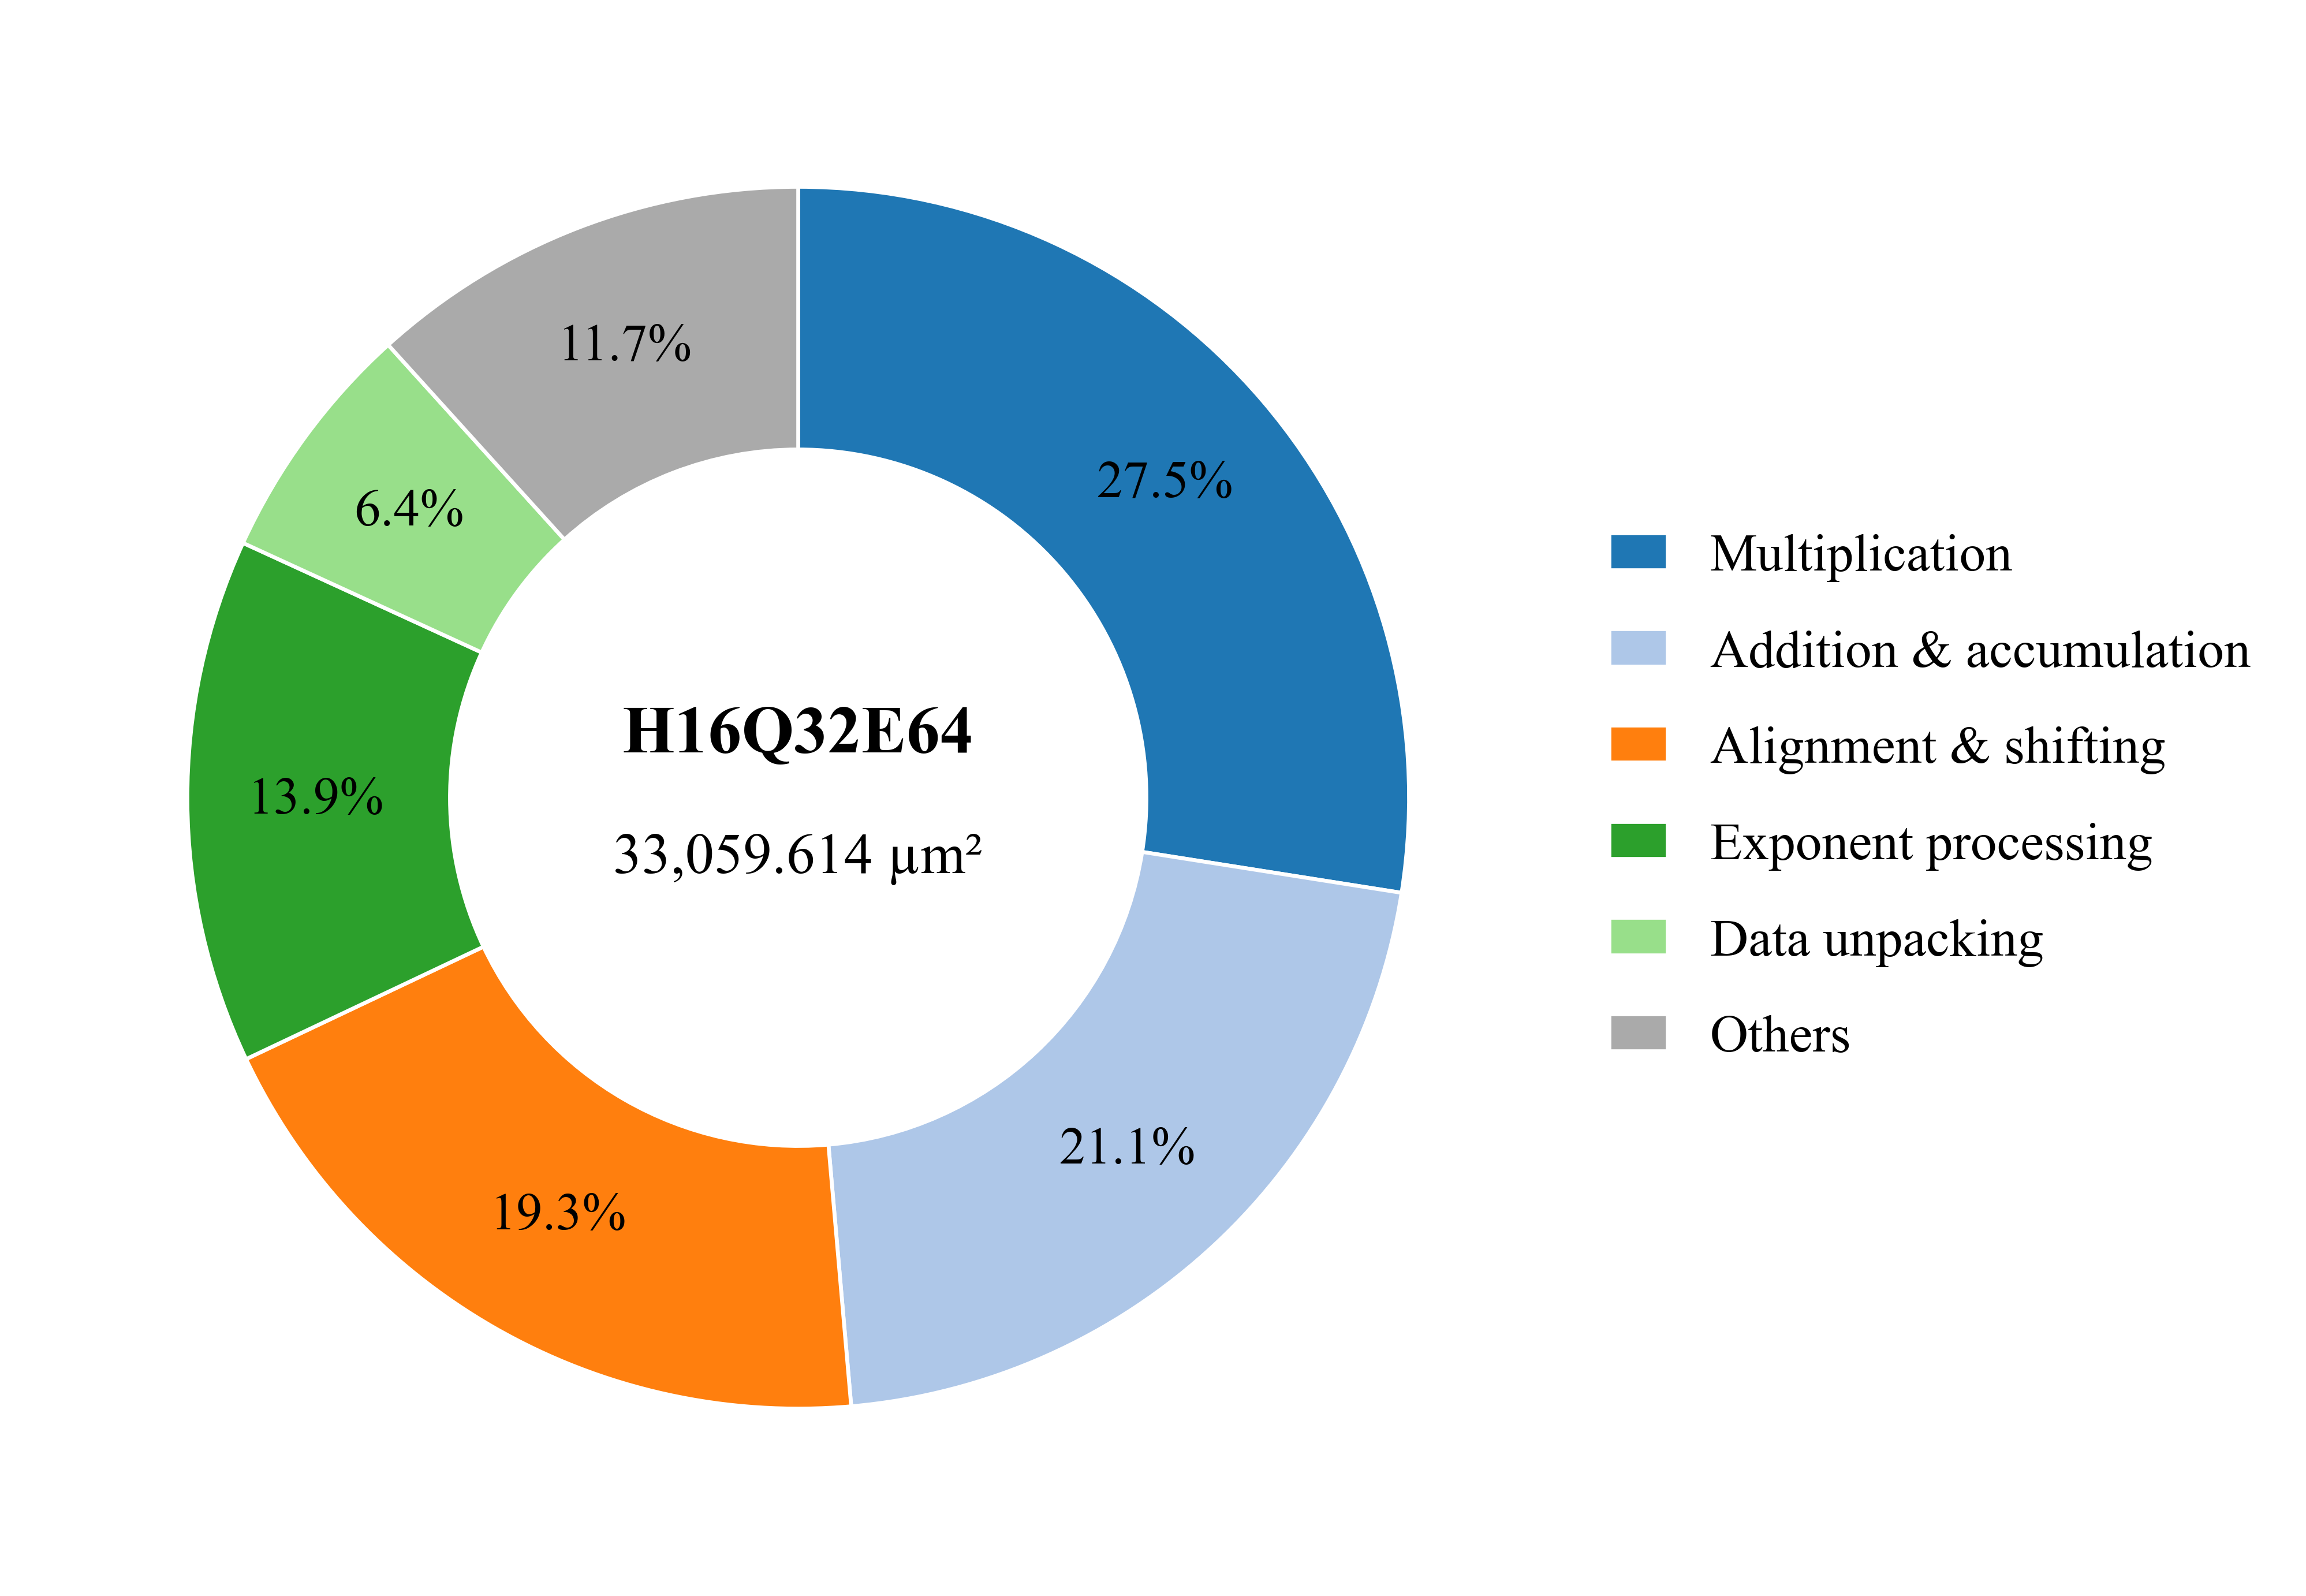
\includegraphics[scale=0.4]{H16Q32E64_area_pie.png}
\caption{Functional area shares of H16Q32E64, including associated registers; denominator: complete DP area.}
\label{fig:full_area_breakdown}
\end{figure}

\subsection{低精度扩展与阵列组织}
\label{sec:kn_evaluation}

\textbf{专用化提高增量算力效率。} 图~\ref{fig:pe_costs_compact} 中，$1:2:8$ 相比 F 增加 34.30\% 面积，将 MXFP4 吞吐提高一倍，每 MAC 能耗降低 23.94\%；$1:2:6$ 的对应能耗降幅为 14.41\%。新增 E 通路的功耗增长小于其吞吐增长，但 FP16/MXFP8 功耗仍增加 2.13\%--2.81\%。因此，低精度扩展的主要收益来自目标模式，未增加算力的模式仍承担附加开销。

\begin{figure}[!t]
\centering
\makebox[\columnwidth][l]{\footnotesize (a) Complete-DP area}\par
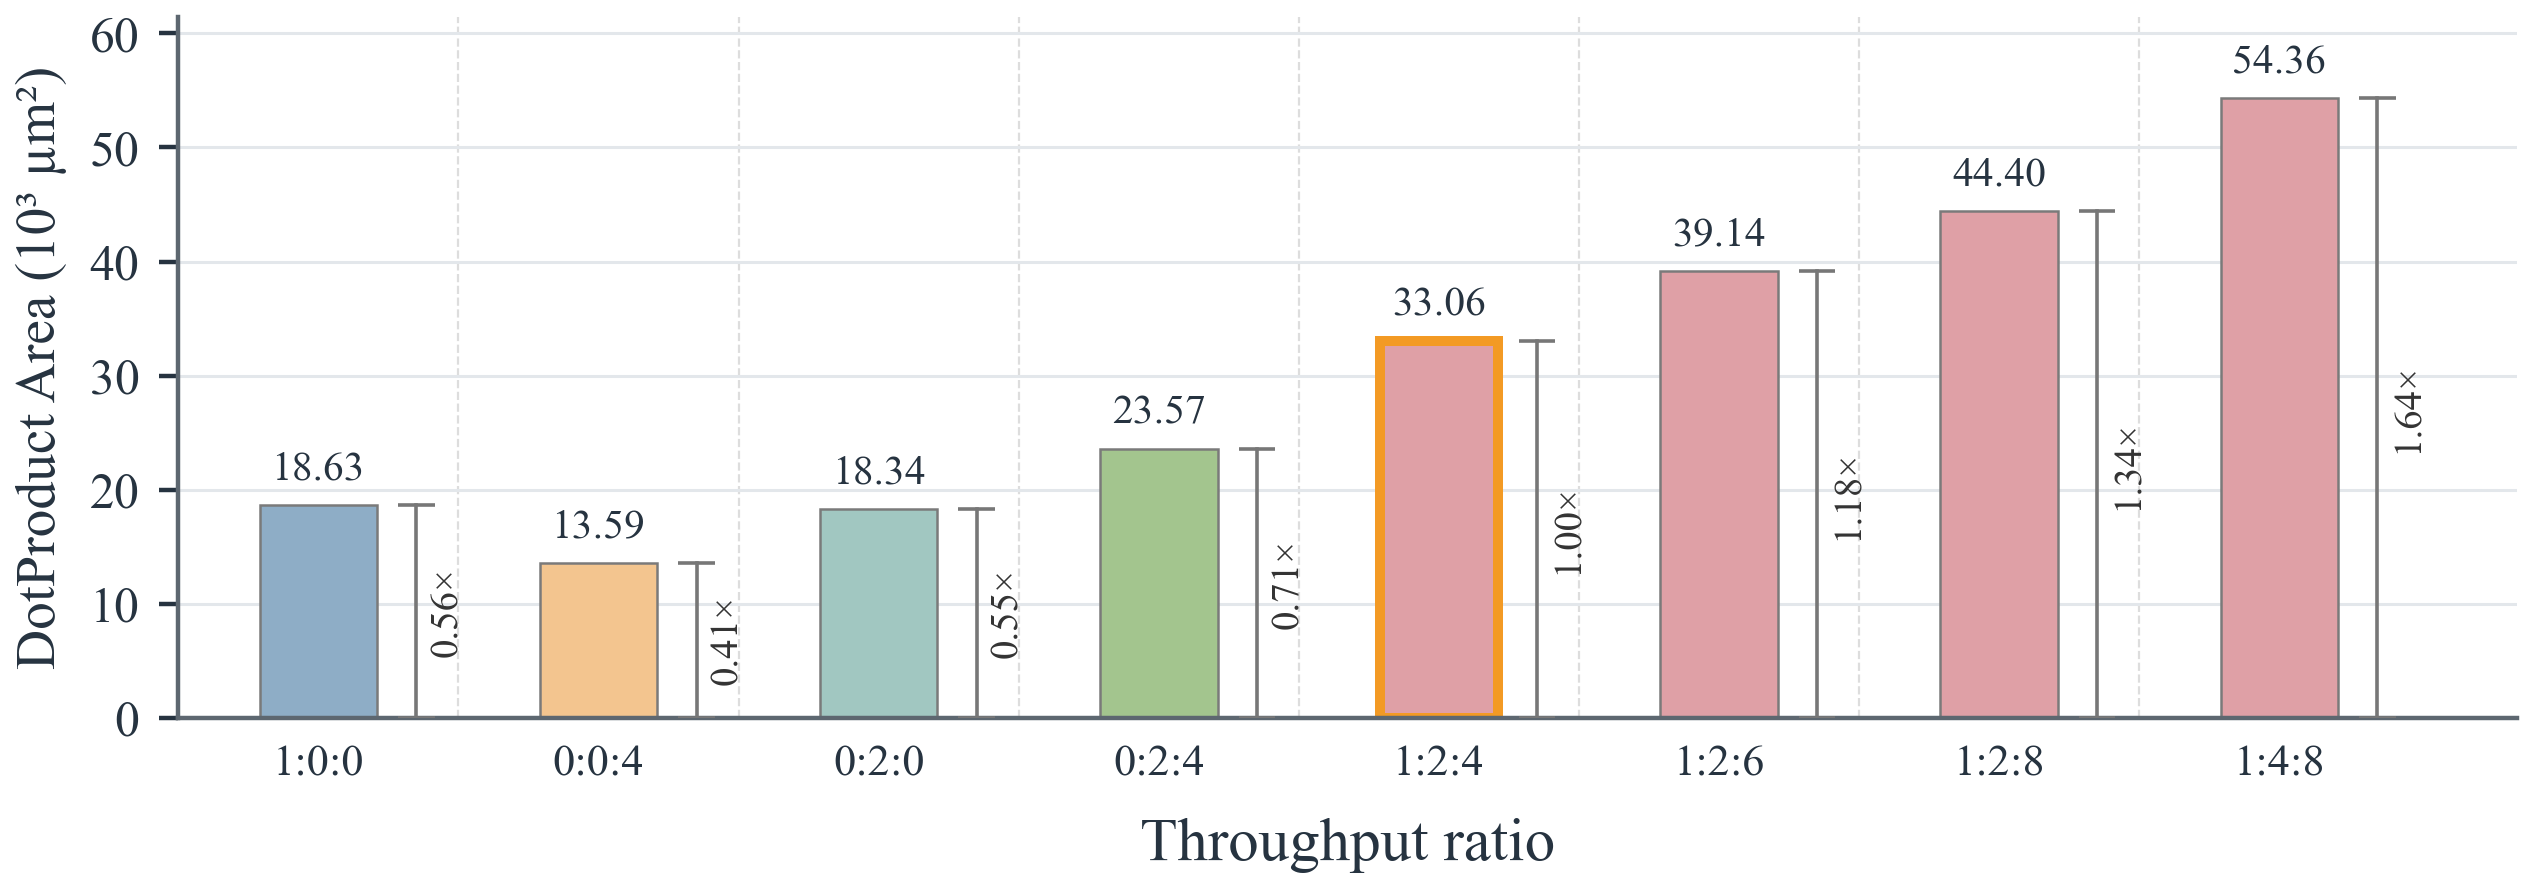
\includegraphics[width=\columnwidth]{selected8_area.png}\par\smallskip
\makebox[\columnwidth][l]{\footnotesize (b) Complete-DP power}\par
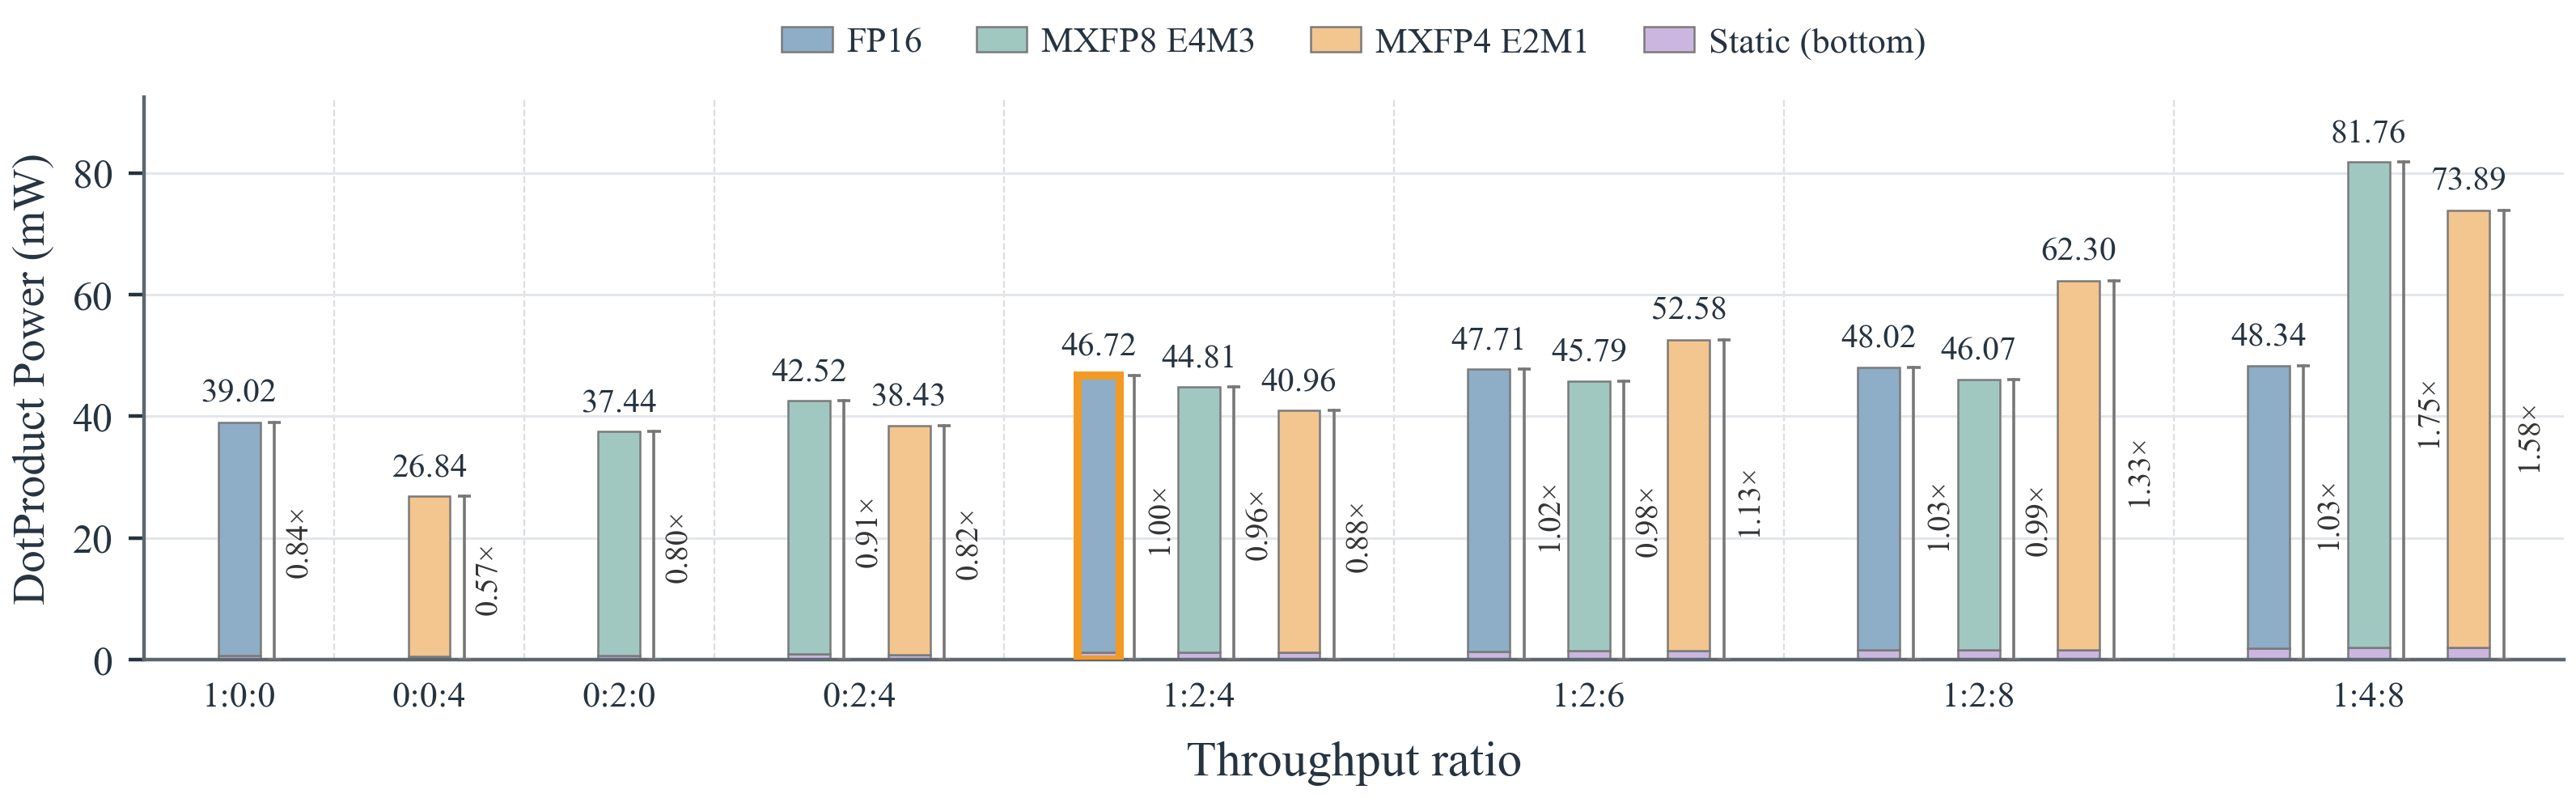
\includegraphics[width=\columnwidth]{selected8_power.png}
\caption{Eight complete-DP costs. Area is relative to F; all power annotations use F--FP16 (46.7175 mW). Power stacks show static and dynamic components for FP16/MXFP8 E4M3/MXFP4 E2M1; zero ratio entries denote unsupported families.}
\label{fig:pe_costs_compact}
\end{figure}

\textbf{共享后端稳定节省面积，能耗收益依赖阵列规模。} 在各精度峰值匹配的 $4\times4$ 基础阵列上，K 组合较 N 组合节省 3.14\%--6.80\% 面积，NVFP4 功耗估计降低 3.79\%--8.03\%（表~\ref{tab:kn_costs}）。扩展到 $16\times4$ 后，K 仍保持面积优势，但 $1:2:6$ 的 NVFP4 功耗估计反而高出 2.01\%。后端共享与新增归约的开销随规模变化，面积收益不能直接外推为能耗收益；在 BF16 模式下，N 关闭附加单元也更有利于抑制功耗。

\begin{table}[t]
\centering
\caption{Estimated K/N costs from a $4\times4$ Full base. Area: mm$^2$; power: W. H/Q/E: BF16/MXFP8 E4M3/NVFP4. N counts active-PE power and inactive leakage.}
\label{tab:kn_costs}
\begingroup\footnotesize\setlength{\tabcolsep}{2.5pt}
\begin{tabular*}{\columnwidth}{@{\extracolsep{\fill}}lcrrrr@{}}\toprule
Ratio & Axis & Area & $P_H$ & $P_Q$ & $P_E$ \\\midrule
$1:2:4$ & K/N & 0.534 & 0.672 & 0.716 & 0.695 \\
$1:2:6$ & K & 0.636 & 0.698 & 0.742 & 0.891 \\
$1:2:6$ & N & 0.656 & 0.679 & 0.721 & 0.926 \\
$1:2:8$ & K & 0.724 & 0.713 & 0.757 & 1.058 \\
$1:2:8$ & N & 0.777 & 0.683 & 0.725 & 1.150 \\
$1:4:8$ & K & 0.883 & 0.718 & 1.306 & 1.238 \\
$1:4:8$ & N & 0.937 & 0.688 & 1.397 & 1.340 \\
\bottomrule
\end{tabular*}\endgroup
\end{table}

\textbf{带宽取舍取决于输出驻留。} 设基础输出形状为 $M\times N$，低精度算力扩展 $r$ 倍，单路输入向量含尺度共 $w$ bit。两方案沿列复用 A、沿行复用 B，每 $\tau$ 次发射交换一次 FP32 C/D。以每次发射的 bit 数计，阵列与本地缓冲间的带宽差为
\begin{equation}
B_N-B_K=(r-1)M\left(\frac{64N}{\tau}-w\right).
\label{eq:kn_bandwidth_difference}
\end{equation}
N 扩列增加 A 的复用，却产生更多独立 C/D 输出；K 扩展减少输出流量，但需要更宽的输入。输出回写频繁时更有利于 K，较长驻留则增强 N 的输入复用收益，与数据流对存储访问成本的影响一致~\cite{timeloop2019}。

按算力密度与单位计算能耗进行 Pareto 比较~\cite{paretomac2025}，四种代表配比在 BF16、MXFP8 和 NVFP4 下的最优者分别为 $1:2:4$、$1:4:8$ 和 $1:2:8$。单精度最优配置并不统一，混合负载的选择还取决于各精度工作量及整核部署成本。

% !TeX root = ../main.tex
\subsection{整核面积约束下的算力分配}
\label{sec:k4_area}

采用 $16\times16$ 阵列，比较四种 $K$ 扩展配比在相同整核面积预算下的部署。H/Q/E 分别以 BF16、MXFP8 E4M3 和 MXFP4 E2M1 为代表格式。华为的 12\,nm RTL 评估中，Cube 簇占 AI Core 面积的 32.7\%，其中计算切片约占 80\%~\cite{luo2024hifloat8area}。据此将基准 DP 阵列的面积占比近似为 $\alpha=0.30$，并采用完整 Ascend 950 架构的 36 个 Cube 单元作为基准数量 $N_0$~\cite{huawei950}。两项数据用于构造等效面积预算，不对应 950 的实际工艺或 die 面积。

令配比 $j$ 的单 DP 面积为 $a_j$，阵列面积 $A_{T,j}=256a_j$，下标 0 表示 $1:2:4$。基准整核面积、固定外围面积及总预算为
\begin{equation}
A_{C,0}=\frac{A_{T,0}}{\alpha},\quad
A_O=A_{C,0}-A_{T,0},\quad
A_{\mathrm{bud}}=N_0A_{C,0}.
\label{eq:k4_area_definition}
\end{equation}
固定每核外围面积 $A_O$，在 $A_{\mathrm{bud}}=405.57$\,mm$^2$ 内重新部署完整核心：
\begin{equation}
n_j=\left\lfloor\frac{A_{\mathrm{bud}}}{A_O+A_{T,j}}\right\rfloor.
\label{eq:core_area_budget}
\end{equation}
设 $m_{j,f}$ 和 $p_{j,f}$ 为单 DP 在精度 $f$ 下的每周期 MAC 数与活动功耗，频率为 $\nu$。按一次 MAC 等于两个 FLOP，部署后的总算力与 DP 功耗为
\begin{equation}
C_{j,f}=2\nu\,256n_jm_{j,f},\qquad
P_{j,f}=256n_jp_{j,f}.
\label{eq:k4_capacity_power}
\end{equation}

表~\ref{tab:k4_absolute} 表明，低精度扩展同时改变单核能力与可部署核心数。$1:4:8$ 将核心数从 36 减至 29，Q 总算力仍提高 61.11\%，H 总算力却下降 19.44\%。因此，低精度加速必须补偿高精度阶段因核心减少而增加的时间，单 DP 峰值不足以判断整核收益。

\begin{table}[!t]
\centering
\caption{Area-constrained N12 deployment. $A_C$: core area (mm$^2$); $C$: TFLOP/s; $P$: DP-only power (W).}
\label{tab:k4_absolute}
\begingroup\footnotesize\setlength{\tabcolsep}{3pt}
% Generated by scripts/reproduce.py.
\begin{tabular*}{\linewidth}{@{\extracolsep{\fill}}lrrcc@{}}\toprule
Ratio & $A_C$ & $n$ & $C_H/C_Q/C_E$ & $P_H/P_Q/P_E$ \\\midrule
$1:2:4$ & 11.266 & 36 & 415.8/831.7/1663.3 & 233.1/232.5/223.3 \\
$1:2:6$ & 12.053 & 33 & 381.2/762.3/2287.0 & 219.3/218.7/260.3 \\
$1:2:8$ & 12.567 & 32 & 369.6/739.2/2957.0 & 210.8/210.1/297.3 \\
$1:4:8$ & 13.615 & 29 & 335.0/1339.9/2679.8 & 192.7/320.1/301.3 \\
\bottomrule\end{tabular*}

\endgroup
\end{table}

\subsection{混合精度负载的性能与能耗}
\label{sec:k4_simplex}

令 $F=\sum_f F_f$ 为 H/Q/E 有效 GEMM 总计算量，$x_f=F_f/F$ 且 $\sum_f x_f=1$。三角坐标表示 FLOP 占比。各精度阶段依次使用全部核心并充分利用对应算力时，计算时间、有效算力和 DP 能耗为
\begin{align}
T_j&=F\sum_f\frac{x_f}{C_{j,f}},&
C_{\mathrm{eff},j}&=\frac{F}{T_j},
\label{eq:k4_time}\\
\mathcal E_j&=F\sum_f x_f\frac{P_{j,f}}{C_{j,f}},&
\varepsilon_{j,f}&=\frac{P_{j,f}}{C_{j,f}}.
\label{eq:k4_energy}
\end{align}
能耗由各精度的计算时间乘对应活动功耗累加，仅计 DP 计算。核心数在单位 FLOP 能耗 $\varepsilon_{j,f}=p_{j,f}/(2\nu m_{j,f})$ 中抵消：增加核心缩短执行时间，却不改变该模型下的单位工作能耗。因此，面积约束通过可部署算力影响时间，而能耗取决于各精度的功耗--吞吐比，两种目标对应不同的最优配比区域。

$T_j$ 和 $\mathcal E_j$ 均为负载组成 $\boldsymbol x$ 的线性函数，候选成本相等处构成分区边界。以 1 个百分点为步长覆盖 5,151 种组成，图~\ref{fig:k4_time_prefill} 分别给出最大有效算力和最低能耗区域，表~\ref{tab:k4_regions} 给出 E 为 MXFP4 时的区域面积占比。

NVFP4 与 MXFP4 共用 E 算力，但单位能耗不同。令 $\rho$ 为 E 工作中 NVFP4 的比例，则 $\varepsilon_{j,E}=(1-\rho)\varepsilon_{j,\mathrm{MX}}+\rho\varepsilon_{j,\mathrm{NV}}$。能耗图的实色区域在两种编码间保持同一最优配比，斜线区域的选择依赖 $\rho$；各模型点按实际编码组成计算能耗。

\begin{figure}[!t]
\centering
\begin{minipage}[t]{0.49\columnwidth}
\centering
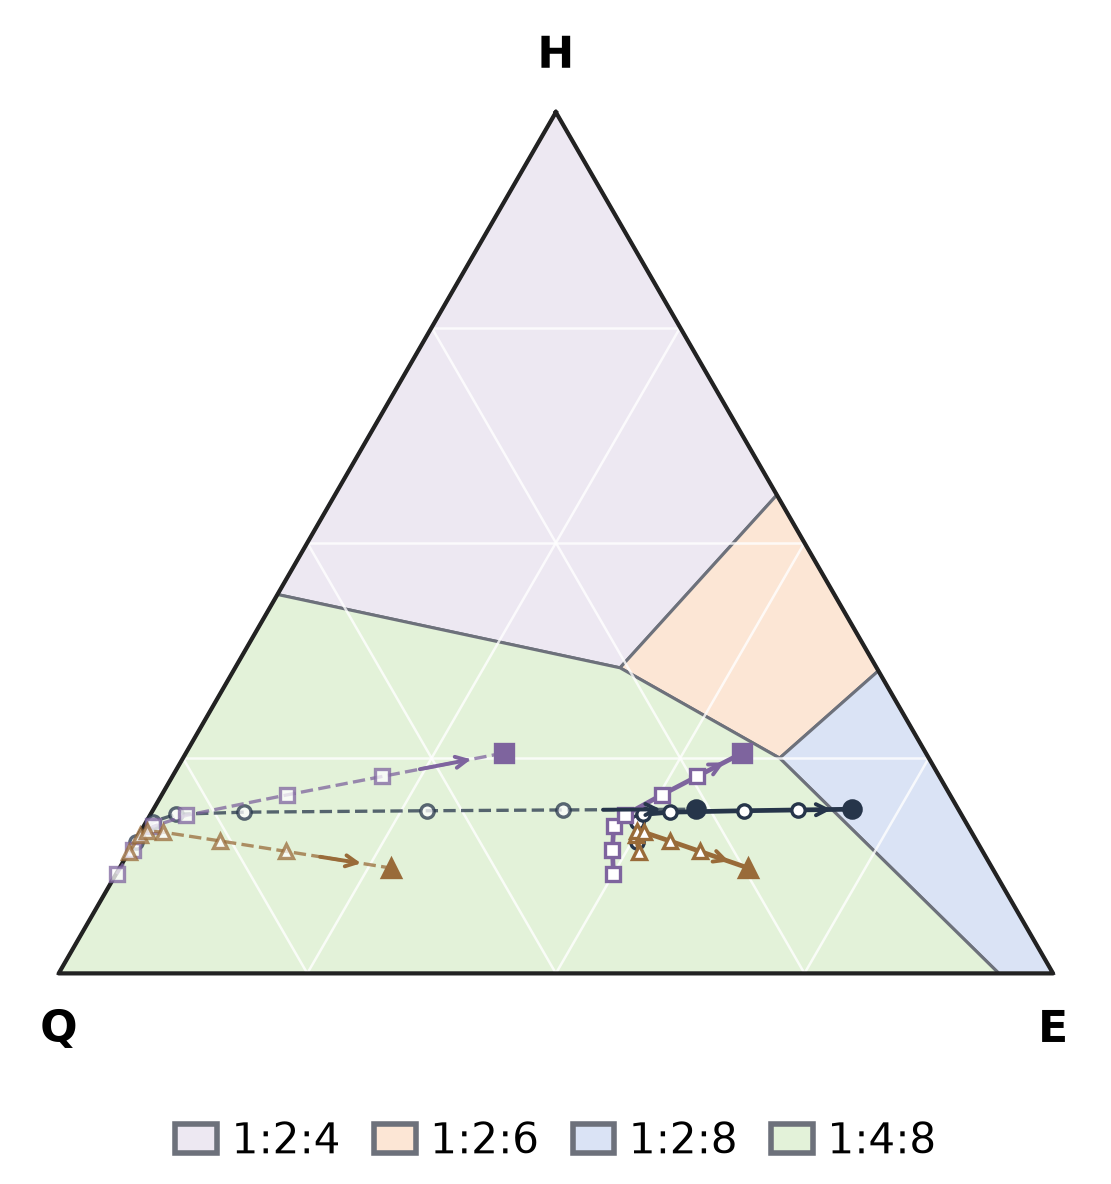
\includegraphics[width=\linewidth]{k4_n12_prefill_time.png}
{\footnotesize (a) Effective throughput\par}
\end{minipage}\hfill
\begin{minipage}[t]{0.49\columnwidth}
\centering
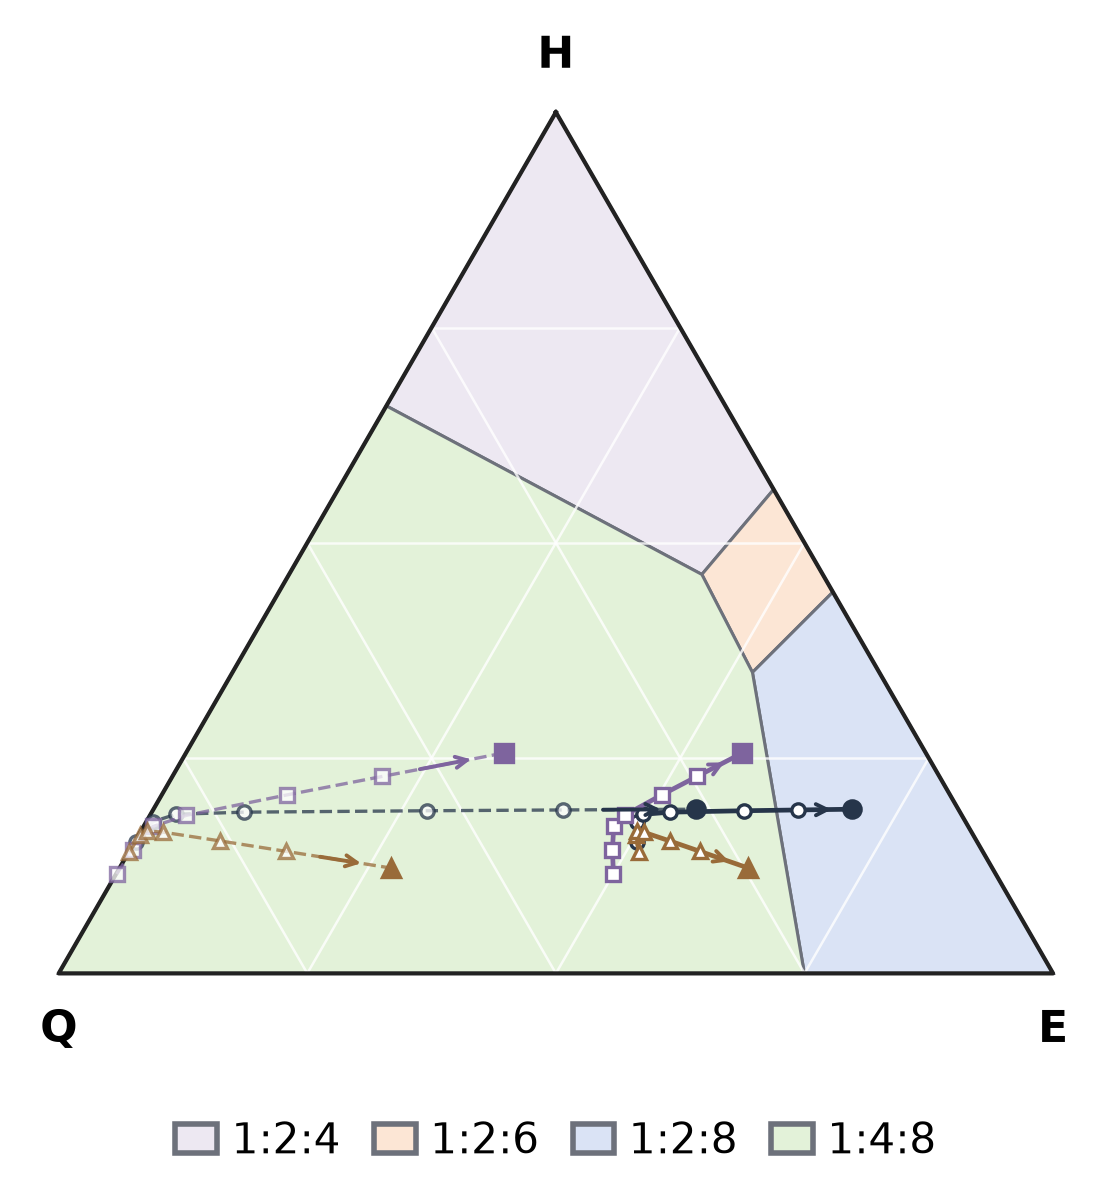
\includegraphics[width=\linewidth]{k4_n12_prefill_energy.png}
{\footnotesize (b) DP compute energy\par}
\end{minipage}
\par\smallskip
{\scriptsize $\circ$ V4-Flash\quad $\square$ V4-Pro\quad $\triangle$ V4.1-Flash\par}
{\scriptsize Dashed: W4A8 experts\quad Solid: NVFP4 W4A4 experts\par}
\caption{Area-constrained ratio selection and prefill trajectories. H/Q/E denote BF16/FP8/FP4 FLOP shares. Arrows follow 1K, 4K, 16K, 64K, 256K, 512K and 1M contexts; filled markers denote 1M. In (b), hatching marks regions whose optimum depends on the MXFP4/NVFP4 mix.}
\label{fig:k4_time_prefill}
\label{fig:k4_energy_prefill}
\end{figure}

\begin{table}[!t]
\centering
\caption{Optimal-region fractions with MXFP4 as E. Energy fractions are unchanged by integer core deployment.}
\label{tab:k4_regions}
\begingroup\footnotesize\setlength{\tabcolsep}{2pt}
% Generated by scripts/reproduce.py.
\begin{tabular*}{\linewidth}{@{\extracolsep{\fill}}lrrr@{}}\toprule
Ratio & Time (cont.) & Time (int.) & DP energy \\\midrule
$1:2:4$ & 31.63\% & 36.85\% & 8.51\% \\
$1:2:6$ & 1.44\% & 0.00\% & 0.00\% \\
$1:2:8$ & 8.44\% & 10.30\% & 23.75\% \\
$1:4:8$ & 58.49\% & 52.85\% & 67.74\% \\
\bottomrule\end{tabular*}

\endgroup
\end{table}

H 密集负载偏向 $1:2:4$，E 密集负载偏向 $1:2:8$，$1:4:8$ 则覆盖较广的混合精度区域。整数部署使 $1:2:6$ 的时间最优区域从连续面积分配下的 1.44\% 消失；其三种精度的单位 FLOP 能耗又均高于 $1:2:8$，因而也不存在能耗最优区域。中间配比并不必然提供独立的负载优势，核心部署粒度和精度相关能效比峰值配比的间隔更具决定性。

\subsection{模型精度需求与配比选择}
\label{sec:k4_prefill}

依据 DeepSeek 的官方配置、推理代码和技术报告~\cite{deepseekv4,deepseekv4flashsource,deepseekv4prosource,deepseekv41source}，分析 V4-Flash、V4-Pro 和 V4.1-Flash 在 batch=1、1K--1M 上下文下的纯文本冷启动 prefill。参考映射将原生 MXFP4 索引点积归入 E，W4A8 路由专家和 FP8 投影归入 Q，BF16 注意力与分组输出投影归入 H。进一步依据已发布的 NVFP4 量化配置~\cite{nvidia2026v4flashnvfp4,nvidia2026v4pronvfp4,nvidia2026deepseeknvfp4}，将路由专家的三个 GEMM 全部映射为 NVFP4 W4A4，其余计算保持不变。同一上下文下，专家量化使 H 不变、Q 向 E 转移。

GEMM 按 $2MNK$ 计数，MoE 仅计激活专家，注意力与索引器遵循因果、窗口、压缩及 top-$k$ 约束。V4.1 进一步计入 CED 的 encoder prefill、decoder 缓存构建和有限窗口重放，并考虑跨层索引复用~\cite{deepseekv41source}。H/Q/E 覆盖所统计 GEMM FLOP 的 97.11\%--99.37\%，其余为 FP32。两个图均叠加参考 W4A8 与专家 W4A4 的上下文轨迹，每种映射包含 21 个点。

\begin{table}[!t]
\centering
\caption{Reference W4A8 prefill endpoints. H/Q/E shares are normalized over useful GEMM FLOPs. Speedup and DP energy reduction $\Delta E$ compare $1:4:8$ against $1:2:4$.}
\label{tab:k4_prefill_points}
\begingroup\footnotesize\setlength{\tabcolsep}{4pt}
% Generated by scripts/reproduce.py.
\begin{tabular*}{\linewidth}{@{\extracolsep{\fill}}llcrr@{}}\toprule
Model & $S$ & $x_H/x_Q/x_E$ (\%) & Speedup & $\Delta E$ (\%) \\\midrule
V4-Flash & 1K & 15.25/84.58/0.17 & 1.274 & 6.77 \\
V4-Flash & 1M & 19.07/26.39/54.55 & 1.138 & 3.93 \\
V4-Pro & 1K & 11.54/88.40/0.06 & 1.335 & 7.49 \\
V4-Pro & 1M & 25.59/42.45/31.96 & 1.098 & 3.75 \\
V4.1-Flash & 1K & 14.08/85.86/0.06 & 1.292 & 7.00 \\
V4.1-Flash & 1M & 12.24/60.49/27.27 & 1.291 & 6.65 \\
\bottomrule\end{tabular*}

\endgroup
\end{table}

\textbf{参考 W4A8 负载受益于 FP8 算力扩展。} 三个模型在短上下文下均以 FP8 计算为主，参考映射的全部采样点在两种目标下均选择 $1:4:8$。V4-Flash 的 E 占比随上下文增长，在 1M 时达到 54.55\%，但 Q 仍占 26.39\%；扩展 FP8 通路的收益足以抵消其相对 $1:2:8$ 的 FP4 算力损失。FP4 工作量占多数尚不足以改变最优配比。

\textbf{上下文增长的影响取决于模型结构。} 参考映射中，V4-Pro 的 H 占比在 1M 时增至 25.59\%，$1:4:8$ 的加速比由 1.335 降至 1.098。V4.1-Flash 则因 CED 与索引复用形成不同轨迹：1M 时 Q 仍占 60.49\%，H 降至 12.24\%，保持 1.291 倍加速和 10.47\% 的 DP 节能（表~\ref{tab:k4_prefill_points}）。高精度注意力、FP8 投影与 FP4 索引计算的相对增长共同决定扩展收益。

\textbf{专家 W4A4 已推动配比转向 $1:2:8$。} 量化后，V4-Flash 的 E 占比由 1K 的 50.52\% 增至 1M 的 70.26\%，Q 则降至 10.68\%。在采样点中，512K 时能耗最优先转向 $1:2:8$，1M 时吞吐也完成切换。V4-Pro 与 V4.1-Flash 在 1M 时仍分别保留 18.46\% 和 24.54\% 的 Q 工作，均选择 $1:4:8$。因此，FP4 专家量化与上下文增长可共同推动配比变化，但剩余 FP8 需求使这种转移具有模型差异。

